\chapter{Sistemi Attivi}
In questo capitolo vengono presentate definizioni, modelli ed esempi riguardanti i sistemi attivi tradizionali.
I sistemi attivi rappresentano una classe specifica di sistemi a eventi discreti. Ad un certo livello di astrazione, generalmente, qualsiasi sistema fisico può essere modellato attraverso un comportamento discreto. Un sistema, infatti, non è continuo o discreto di per sé, anche se si può prestare o meno ad una certa scelta nel modello da adottare.
I sistemi attivi sono asincroni; questo significa che gli eventi generati dai componenti sono immagazzinati nei link prima di essere consumati (in maniera asincrona).
Il modello dei sistemi attivi include due tipi fondamentali di elementi: i componenti e i link. Un sistema attivo è una rete di componenti connessi gli uni agli altri per mezzo di link uscenti da terminali di output di alcuni componenti ed entranti nei terminali di input di altri componenti. Il comportamento di ogni componente è descritto da un automa a stati finiti, le cui transizioni tra gli stati sono compiute in base alla consumazione di determinati eventi disponibili nei terminali di input. L'esecuzione di una transizione causa la generazione di eventi trasmessi ai terminali di output del componente. \'E altresì possibile che alcune transizioni non vengano innescate da alcun evento particolare presente nel modello: in questo caso si assume che l'evento scatenante provenga dal mondo esterno al sistema. Il modello comportamentale del componente è assunto essere completo, nel senso che racchiude sia le transizioni normali, sia quelle di guasto.
Un sistema attivo è quindi caratterizzato da una topologia (collegamenti tra componenti) e dal comportamento dei singoli componenti e dei link. Questi ultimi, in un problema generale, potrebbero avere differenti capacità di immagazzinamento (in termini di numero di eventi) e comportamenti diversi nel caso siano colmi (la cosiddetta politica di saturazione).
Il modello globale del sistema è quindi implicitamente dato dalla topologia dell'insieme e dai comportamenti dei singoli componenti e dei link. 

\newpage
\section{Definizioni}
\subsection{Componenti} 
I componenti sono i costituenti base dei sistemi attivi. Ogni componente è caratterizzato da due modelli:
\begin{enumerate}
\item \emph{modello topologico}, secondo il quale un componente è descritto da un insieme di terminali di input, da cui gli eventi in ingresso sono consumati, e da un insieme di terminali di output, dai quali gli eventi in uscita sono generati;
\item \emph{modello comportamentale}, descritto da un automa a stati finiti che ingloba sia il comportamento normale sia le transizioni di guasto, dotato di una funzione di transizione che mappa uno stato e un evento in ingresso in un nuovo stato, generando un sottoinsieme (eventualmente vuoto) di eventi nei terminali di uscita.  
\end{enumerate}

\begin{defn}
Un modello di un componente è un automa:
\begin{center}
	$M_c = (S,E_{in},I,E_{out},O,\tau)$
\end{center}
dove $S$ è l'insieme degli stati, $E_{in}$ è l'insieme degli eventi in ingresso, $I$ è l'insieme dei terminali di input, $E_{out}$ è l'insieme degli eventi in uscita, $O$ è l'insieme dei terminali di output, e $\tau$ è la funzione di transizione (non deterministica):
\begin{center}
	$ \tau : S \times (E_{in} \times I) \times 2^{(E_{out} \times O)} \rightarrow 2^S $.
\end{center}

Un evento è una coppia $(e,\theta)$, dove $e$ è un ingresso (uscita) e $\theta$ un terminale di ingresso (uscita). Un componente particolare può essere visto come una istanza di un modello di componente. 
Una transizione $t$ da uno stato $s$ ad uno stato $s^\prime$ è innescata da un evento in ingresso $(e,x)$ disponibile al terminale di input $x$ e genera l'insieme (possibilmente vuoto) di eventi 
$\{(e_1,y_1), \ldots ,(e_n,y_n)\}$ in corrispondenza dei terminali di output $y_1, \ldots,y_n$, in simboli:
\begin{center}
	$t = s \xrightarrow {(e,x) \Rightarrow (e_1,y_1), \ldots ,(e_n,y_n)} s^{\prime}$.
\end{center}
\end{defn}
\'E implicitamente definito un terminale di input virtuale, chiamato $In$, attraverso il quale giungono gli eventi esterni al sistema.

\begin{ex}\label{ex:modelli}
Si consideri l'esempio di un sistema attivo costituito da un meccanismo di protezione per una linea elettrica. Il componente $p$ rappresenta la protezione (\emph{protection device}), ovvero un sensore che si attiva quando rileva bassa tensione ai capi della linea. Il componente $b$ rappresenta il \emph{breaker}, ovvero il dispositivo che, comandato dalla protezione, si apre isolando la linea elettrica e prevenendo il cortocircuito, oppure si chiude riconnettendo la rete. Nella figure \ref{fig:model_p} e \ref{fig:model_b}  sono rappresentati, rispettivamente, i modelli relativi alla protezione e quelli riferiti al breaker.
Il componente di protezione non possiede terminali di input e ha un terminale di output $o$, mentre il breaker dispone solamente di un terminale di input $i$.
La protezione può essere nello stato inattivo \emph{idle} quando non viene rilevato alcun cortocircuito, oppure nello stato \emph{awaken}, nel momento in cui la tensione si abbassa oltre una certa soglia. Quando viene rilevato un cortocircuito, il componente $p$ può compiere le transizioni $p_1$, che genera un evento $op$ per comandare l'apertura del breaker, o $p_3$, che a causa di un malfunzionamento genera invece un evento $cl$ per comandare la chiusura del breaker. Quando il cortocircuito svanisce, il componente torna nello stato $idle$ percorrendo la transizione $p_2$, che genera l'evento $cl$, oppure tramite $p_4$, che genera in maniera difettosa l'evento $op$.
Il breaker può essere aperto ($open$) o chiuso ($closed$). Quando è chiuso e un evento $op$ è disponibile in corrispondenza del terminale $i$, il breaker $b$ può percorrere la transizione $b_1$ che lo apre o $b_3$ con la quale resta chiuso (guasto). Quando il componente è aperto, le transizioni possibili sono $b_2$ se il breaker si apre, $b_4$ se a causa di un guasto rimane chiuso. Le transizioni $b_5$ e $b_6$ non cambiano lo stato del componente.
Un sunto delle transizioni relative ai due componenti è fornito nelle tabelle \ref{tab:p_trans} e \ref{tab:b_trans}.
\end{ex}

\begin{figure}[htbp]
\centering
\subfigure[topologia protezione]
{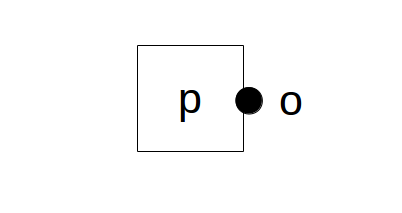
\includegraphics[scale=0.4]{./Img/sa/top_protection.png}}
\hspace{10mm}
\subfigure[comportamento protezione]
{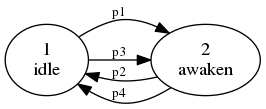
\includegraphics[scale=0.5]{./Img/sa/model_protection.png}}
\caption{Modello del componente $p$}
\label{fig:model_p}
\end{figure}

\begin{figure}[htbp]
\centering
\subfigure[topologia breaker]
{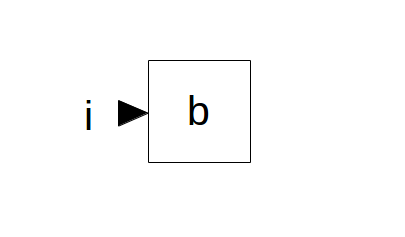
\includegraphics[scale=0.4]{./Img/sa/top_breaker.png}}
\hspace{10mm}
\subfigure[comportamento breaker]
{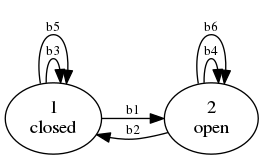
\includegraphics[scale=0.5]{./Img/sa/model_breaker.png}}
\caption{Modello del componente $b$}
\label{fig:model_b}
\end{figure}

\begin{table}[htbp] 
\begin{tabularx}{\textwidth}{l X}
\hline
\textbf{Transizione} & \textbf{Descrizione}\\
\hline\\
$p_1 = idle \xrightarrow{(sh,In) \Rightarrow (op,o)} awaken$ & Rileva un cortocircuito e genera l'evento $op$\\[1mm]
$p_2 = awaken \xrightarrow{(ok,In) \Rightarrow (cl,o)} idle$ & Rileva la fine del cortocircuito e genera l'evento $cl$\\[1mm]
$p_3 = idle \xrightarrow{(sh,In) \Rightarrow (cl,o)} awaken$ & Rileva un cortocircuito ma genera l'evento $cl$\\[1mm]
$p_4 = awaken \xrightarrow{(ok,In) \Rightarrow (op,o)} idle$ & Rileva la fine del cortocircuito ma genera l'evento $op$\\[1mm]
\hline
\end{tabularx}
\caption{Transizioni relative alla protezione}
\label{tab:p_trans}
\end{table}

\begin{table}[htbp] 
\begin{tabularx}{\textwidth}{l X}
\hline
\textbf{Transizione} & \textbf{Descrizione}\\
\hline\\
$b_1 = closed \xrightarrow{(op,i)} open$ & Consuma l'evento $op$ e apre\\[1mm]
$b_2 = open \xrightarrow{(cl,i)} closed$ & Consuma l'evento $cl$ e chiude\\[1mm]
$b_3 = closed \xrightarrow{(op,i)} closed$ & Consuma l'evento $op$ ma rimane chiuso\\[1mm]
$b_4 = open \xrightarrow{(cl,i)} open$ & Consuma l'evento $cl$ ma rimane aperto\\[1mm]
$b_5 = closed \xrightarrow{(cl,i)} closed$ & Consuma l'evento $cl$\\[1mm]
$b_6 = open \xrightarrow{(op,i)} open$ & Consuma l'evento $op$\\[1mm]
\hline
\end{tabularx}
\caption{Transizioni relative al breaker}
\label{tab:b_trans}
\end{table}

\subsection{Link}
Nell'ambito dei sistemi attivi, i componenti sono tra loro connessi per mezzo di link. Ogni link esce da un terminale di output $y$ di un componente $c$ e entra in un terminale di input $x$ di un componente $c^\prime$.
Analogamente a quanto avviene per i componenti, anche i link sono caratterizzati da un modello, che costituisce un'astrazione del link specifico appartenente al sistema.

\begin{defn}
Un modello di un link è una quadrupla
\begin{center}
	$M_l = (x,y,z,w)$
\end{center}
dove $x$ è il terminale di input, $y$ il terminale di output, $z$ la dimensione e $w$ la politica di saturazione.
\end{defn}
Un particolare link $l$ è un'istanza di un modello siffatto, e consiste quindi in un canale di comunicazione unidirezionale fra due componenti distinti $c$ e $c^\prime$, dove un terminale di output $y$ di $c$ e un terminale di input $x$ di $c^\prime$ coincidono rispettivamente con l'input e l'output del link $l$.
La dimensione $z$ rappresenta il numero massimo di eventi che possono essere accodati nel link. 
Indichiamo con $|l|$ la configurazione corrente del link. 
Se il numero di eventi attualmente memorizzati coincide con la dimensione, il link si dice essere saturo.
Quando il link è saturo, la semantica legata al compimento delle transizioni è dettata dalla politica di saturazione $w$, la quale può essere:
\begin{itemize}
\item \emph{lose}: l'evento, non potendo essere memorizzato, viene perso;
\item \emph{override}: l'evento sovrascrive l'ultimo evento nel link;
\item \emph{wait}: la transizione non viene portata a termine fintanto che il link permane nello stato di saturazione, ovvero fino a quando almeno un evento nel link non viene consumato.
\label{saturation}
\end{itemize}
Nell'ambito di questa tesi, si considererà il caso particolare di link di dimensione unitaria e politica di saturazione $wait$ , ovvero $z = 1$ e $w = wait$.
Tale supposizione permette di visualizzare le configurazioni dei link dell'intero sistema come la tupla del contenuto dei terminali di input di ogni componente del sistema. Implicitamente questo significa che ogni evento generato è inserito istantaneamente, se libero, nel terminale (o nei terminali) di input liberi collegati al terminale di output. Se un terminale di destinazione è occupato, la transizione non viene compiuta.

\begin{ex}\label{ex:link}
Con riferimento all'esempio \ref{ex:modelli}, in figura \ref{fig:model_link} è presentato il link $pb$ che collega il terminale di output $o$ della protezione $p$ al terminale di input $i$ del breaker $b$.
\end{ex}

\begin{figure}[htbp]
\centering
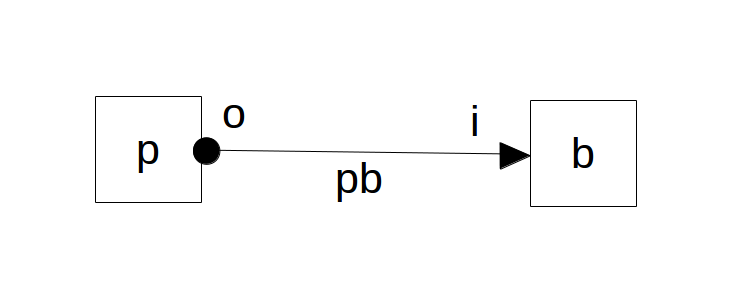
\includegraphics[scale=0.4]{./Img/sa/link.png}
\caption{Modello del sistema attivo $\overline{A}$}
\label{fig:model_link}
\end{figure}

\subsection{Sistema attivo}
Un sistema attivo è una rete di componenti interconnessi per mezzo di link. Ogni componente ed ogni link del sistema sono caratterizzati da un modello e quindi, in generale, più elementi potrebbero avere il medesimo modello. Si assume che più link possano uscire da un terminale di output di un componente, mentre al massimo un link possa entrare in un terminale di input.
Un sistema potrebbe contenere dei terminali che non sono connessi con alcun link: questi vengono chiamati terminali scollegati.

\begin{defn}
Un sistema attivo è una tripla
\begin{center}
	$ A = (C,L,D)$
\end{center}
dove $C$ è l'insieme dei componenti, $L$ l'insieme dei link tra terminali di componenti in $C$, e $D$ è l'insieme dei terminali scollegati. Quest'ultimo insieme può essere visto come l'unione di due insiemi disgiunti:
\begin{center}
	$ D = D_{on} \cup D_{off}$
\end{center}
dove $D_{on}$ è l'insieme dei terminali on scollegati, mentre $D_{off}$ è l'insieme dei terminali off scollegati. 
\end{defn}
Se $D_{on} \neq \emptyset $, il sistema $A$ è detto aperto, altrimenti è detto chiuso. Nel caso $A$ sia chiuso ($D_{on} = \emptyset$), nessun evento è disponibile nei terminali di input di $D_{off}$, mentre gli eventi generati nei terminali di output di $D_{off}$ sono persi.
D'altro canto, se $A$ è aperto, si assume che i terminali scollegati in $D_{on}$ siano connessi attraverso link all'esterno del sistema $A$; quest'ultimo, in altre parole, è come se fosse incorporato in un altro sistema più grande (sconosciuto). Quindi gli eventi generati in terminali di output in $D_{on}$ sono immagazzinati all'interno dei link (sconosciuti) esterni al sistema $A$. Analogamente, il componente in corrispondenza del quale si trova un terminale di input in $D_{on}$ è sensibile a eventi disponibili in quel terminale.

\begin{ex} \label{ex:sa}
Con riferimento agli esempi \ref{ex:modelli} e \ref{ex:link}, il sistema rappresentato in figura \ref{fig:model_link} è un sistema attivo $\overline A = (\{p,b\},\{pb\},\emptyset)$ nel quale non è presente alcun terminale scollegato.
\end{ex}

\subsection{Traiettoria}
Un sistema attivo può essere pensato come una macchina che può essere in uno stato quiescente o in uno stato reattivo. Se si trova nello stato quiescente, i componenti non effettuano alcuna transizione, dal momento che nessun evento è disponibile nei terminali di ingresso. In corrispondenza del verificarsi di un determinato evento, sia esso proveniente dal mondo esterno, sia da un terminale di input scollegato appartenente a $D_{on}$, il sistema evolve nella sua fase reattiva. Dato che il comportamento del sistema è asincrono (non dipende dal tempo), la reazione, detta \emph{traiettoria} (o \emph{storia}), consiste in una sequenza di transizioni compiute da componenti presenti nel sistema.
Ogni transizione di un componente porta il sistema in un nuovo stato, dove uno stato è identificato dallo stato corrente di ogni componente e dallo stato attuali di ogni link. In altre parole, uno stato del sistema attivo è una coppia $(S,Q)$, dove $S$ è la n-pla degli stati dei componenti, mentre $Q$ è la m-pla delle configurazioni dei link, ovvero la m-pla del contenuto dei terminali di input di tutti i componenti.
In questo lavoro di tesi, il focus è sulla cosiddetta diagnosi a posteriori, che avviene quando il sistema ha percorso una traiettoria partendo da uno stato quiescente e tornando in uno stato di quiete, nel quale cioè tutti i terminali di input dei componenti sono vuoti. In questo contesto, una traiettoria completa può essere vista come una sequenza di transizioni che, partendo dallo stato iniziale (quiescente), termina in uno stato finale (anch'esso quiescente).
Una transizione del sistema può essere scritta come:
\begin{center}
	$T = (S,Q) \xrightarrow {t(c)} (S^\prime,Q^\prime)$,
\end{center}
dove $t(c)$ identifica univocamente la transizione $t$ appartenente al modello del componente $c$.
Assumendo che $a_0 = (S_0,Q_0)$ sia lo stato iniziale del sistema, la traiettoria ottenuta partendo da $a_0$ è la sequenza di stati del sistema determinata dall'occorrenza di transizioni $t_1, \ldots , t_k$ attuabili da parte dei singoli componenti:
\begin{center}
$h = a_0 \xrightarrow{t_1(c_1)} a1 \xrightarrow{t_2(c_2)} a2 \ldots \xrightarrow{t_k(c_k)} a_k$.
\end{center}
Ogni stato (non iniziale) dipende quindi dallo stato precedente e dalla particolare transizione che lo porta allo stato corrente, ovvero la coppia $(a_{i-1},t_i(c_i))$. Assumendo che si parta dallo stato iniziale $a_0$ questo ci permette di identificare una traiettoria per mezzo delle sole transizioni dei componenti:
\begin{center}
$h = [t_1(c_1),t_2(c_2), \ldots , t_k(c_k)]$.
\end{center}

\begin{ex} \label{ex:traiettoria}
Con riferimento al sistema attivo in figura \ref{fig:model_link}, si assuma che lo stato iniziale sia la composto dalla tripla $(idle,closed,\epsilon)$ indicante rispettivamente gli stati dei componenti $p$ e $b$ (figure \ref{fig:model_p} e \ref{fig:model_b}) e il contenuto inizialmente vuoto del link $pb$, ovvero del terminale di input $i$ del breaker. Una possibile traiettoria è la seguente:
\begin{center}
$\overline h = (idle,closed,\epsilon) \xrightarrow{p_1(p)} (awaken,closed,op) \xrightarrow{b_1(b)}(awaken,open,\epsilon) \xrightarrow{p_2(p)} (idle,open,cl) \xrightarrow{b_2(b)} (idle,closed,\epsilon)$
\end{center}
che corrisponde alla seguente dinamica:
\begin{enumerate}
\item la protezione rileva un cortocircuito e comanda l'apertura del breaker;
\item il breaker si apre;
\item la protezione rileva la fine del cortocircuito e comanda la chiusura del breaker;
\item il breaker di chiude.
\end{enumerate}
Si noti come lo stato finale della traiettoria $\overline{h}$ coincida con lo stato iniziale della medesima traiettoria. Questa ciclicità permette di inferire la presenza di infinite traiettorie per il sistema attivo in esame, in quanto percorrere un ciclo un diverso numero di volte porta alla percorrenza di traiettorie diverse.
Da osservare, inoltre, come una siffatta dinamica sia esente da guasti: nelle sezioni successive verranno analizzati casi più generali, contraddistinti da malfunzionamenti, e saranno fornite le informazioni necessarie al fine di discriminare le transizioni normali da quelle di guasto.
\end{ex}

\subsection{Behavior Space}
Dato un sistema attivo ed il suo stato iniziale, possono esservi molte traiettorie percorribili, persino infinite. Analogamente a quanto avviene per il comportamento del singolo componente, che può essere descritto nel suo modello come un automa a stati finiti, anche per quanto riguarda le traiettorie dell'intero sistema si può seguire un procedimento analogo. Un automa a stati finiti rappresenta infatti, attraverso un numero di stati e di transizioni finiti, un numero di traiettorie che può essere infinito. Questo è dovuto alla possibile presenza di ciclicità all'interno dell'automa. Tale automa è chiamato \emph{behavior space} e ha come alfabeto l'intero insieme delle transizioni dei singoli componenti del sistema.
Il linguaggio del \emph{behavior space} $Bsp(A)$ con stato iniziale $a_0$ coincide con l'insieme di tutte le possibili traiettorie del sistema $A$ partendo dallo stato $a_0$. 
\begin{defn}
Sia $A = (L,C,D)$ un sistema attivo, dove $C$ è l'insieme di $n$ componenti, mentre $L$ è l'insieme di $m$ link. Il behavior space di $A$ è il DFA
\begin{center}
	$Bsp(A) = (\Sigma,\alpha,\tau,a_0,\alpha_f)$
\end{center}
dove:
\begin{enumerate}
\item $\Sigma$ è l'alfabeto, dato dall'unione delle transizioni dei componenti in $C$;
\item $\alpha$  è l'insieme degli stati $(S,Q)$, con $S = (s_1,\ldots,s_n)$ una n-pla di stati dei componenti in $C$, e $Q = (q_1, \ldots,q_m)$ una m-pla del contenuto dei terminali di input di tutti i componenti;
\item $a_0 = (S_0,Q_0)$ è lo stato iniziale;
\item $\alpha_f$ è l'insieme degli stati finali, ovvero stati in cui $Q = (\epsilon \ldots \epsilon)$;
\item $\tau$ è la funzione di transizione deterministica, $\tau: \alpha \times \Sigma \rightarrow \alpha$, tale che $(S,Q) \xrightarrow{t(c)} (S^\prime, Q^\prime) \in \tau$, dove $S = (s_1, \ldots,s_n)$, $Q = (q_1, \ldots,q_m)$, $S^\prime = (s^\prime_1, \ldots,s^\prime_n)$, $Q^\prime = (q^\prime_1, \ldots,q^\prime_m)$ e
\begin{center}
$t(c) = s \xrightarrow{(e,x) | \{(e_1,y_1), \ldots, (e_p,y_p)\}} s^\prime$
\end{center}
se e solo se:
\begin{itemize}
\item $x = In$, cioè l'evento è disponibile sul terminale di input virtuale sensibile agli eventi esterni al sistema, oppure $x \in D_{on}$, o $e$ è pronto al terminale $x$ all'interno di un link del sistema;
\item Per ogni $i \in [1 \ldots n]$, abbiamo
\begin{center}
$s^\prime_i = \begin{cases} s^\prime & \mbox{se }c_i = c\\ s_i & \mbox{altrimenti} \end{cases}$
\end{center}
cioè per ogni transizione del \emph{behavior space} cambia lo stato relativo al singolo componente coinvolto nella transizione;
\item $Q^\prime$ differisce da $Q$ per le seguenti condizioni:
\begin{itemize}
\item $Q(x) = e \rightarrow Q^\prime(x) = \epsilon$, cioè l'evento in input è consumato;
\item $\forall(e_j,y_j), j \in [1 \ldots p], Q(y_j) = \epsilon \rightarrow Q^\prime(y_j) = e_j$, cioè gli eventi di uscita sono inseriti nei terminali di input connessi ai terminali di output coinvolti nella transizione. 
\end{itemize}
\end{itemize}
\end{enumerate}
\end{defn}
Il \emph{behavior space}, contenendo tutte le possibili traiettorie del sistema, assume dimensioni considerevoli anche con la presenza di pochi componenti e relativi terminali di input. Questo perché la sua dimensione ha una complessità esponenziale nel numero di componenti e link, dato che uno stato del \emph{behavior space} è caratterizzato, nel caso peggiore, da tutte le possibili combinazioni di stati dei componenti e contenuto dei link \footnote{Si tratta di un limite di complessità superiore. In base alle particolari transizioni coinvolte, infatti, non tutte le combinazione sono possibili stati del \emph{behavior space}.}. Per questo motivo, si assume che un automa siffatto non possa essere generato perché troppo costoso, in termini di tempo di esecuzione ma soprattutto di memoria. Nella risoluzione del problema di diagnosi, infatti, verrà generato un automa più contenuto, chiamato semplicemente \emph{behavior}.

\begin{ex}
Il \emph{behavior space} del sistema attivo $\overline{A}$ dell'esempio \ref{ex:sa} è riportato in figura \ref{fig:bsp}. Si considera come stato iniziale $a_0$ lo stato nel quale la protezione è inattiva, il breaker è chiuso e il link $pb$ è vuoto. Gli archi evidenziati rappresentano la particolare traiettoria $\overline{h}$ introdotta nell'esempio \ref{ex:traiettoria}, mentre i nodi con un doppio contorno rappresentano gli stati finali $\alpha_f$ nei quali l'unico link $pb$ del sistema è vuoto.
\end{ex}

\begin{figure}[htbp]
\centering
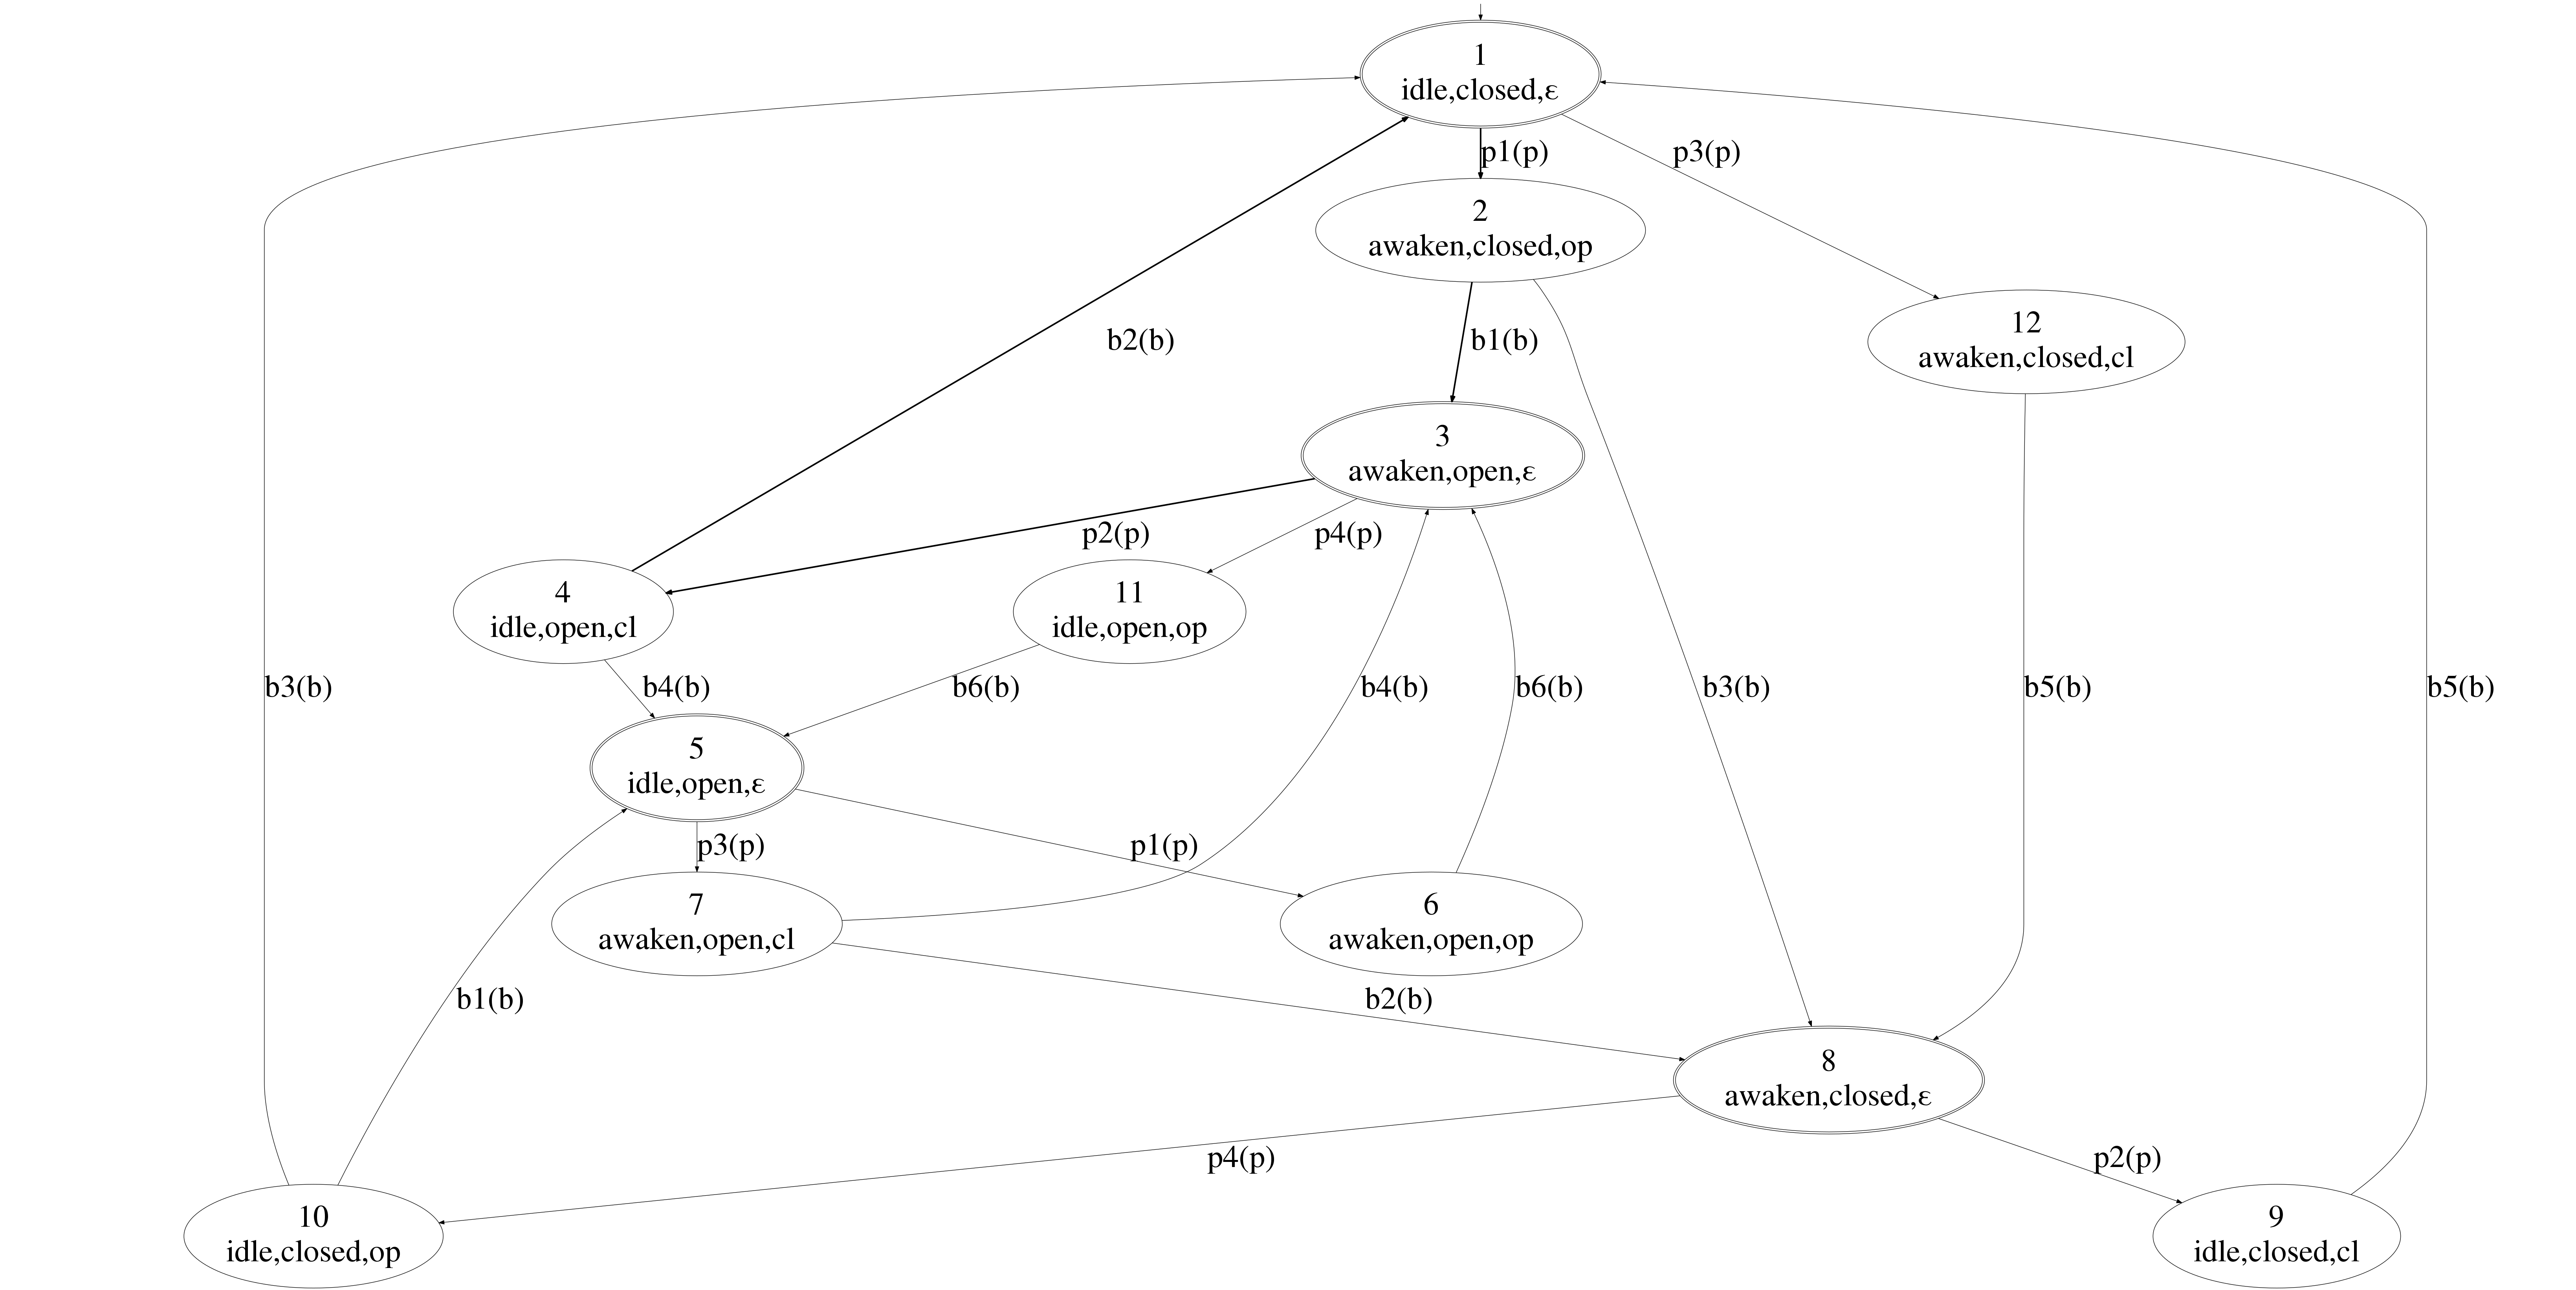
\includegraphics[scale=0.11]{./Img/sa/behavior_space.png}
\caption{Behavior space del sistema attivo $\overline{A}$}
\label{fig:bsp}
\end{figure}

\newpage
\section{Problema diagnostico}
Un sistema attivo, inizialmente, si trova in uno stato quiescente, ovvero in uno stato in cui i link sono vuoti. Il sistema passa alla fase reattiva nel momento in cui riceve dei particolari eventi esterni. Una volta che l'occorrenza di un tale evento si verifica, la reazione del sistema è composta da una sequenza di transizioni che formano una traiettoria. Dato che ogni componente è modellato dal suo comportamento completo, ovvero sia dai suoi comportamenti normali sia quelli di guasto, sono necessarie delle informazioni aggiuntive, in grado di determinare se le transizioni facenti parte della traiettoria siano di guasto o normali. Un ulteriore problema consiste nella non completa osservabilità tipica dei sistemi reali: una traiettoria, in generale, non è percepita come effettivamente è, ma quello che è visibile consiste in una proiezione di un suo sottoinsieme osservabile. Una sequenza di label osservabili costituisce una traccia della reale traiettoria. Inoltre, una label associata ad una transizione di un componente potrebbe non identificare univocamente la transizione, poiché più transizioni possono condividere la medesima label di osservazione. Si noti come i modelli comportamentali dei singoli componenti non effettuino una distinzione tra ciò che osservabile e quello che non lo è: per questo motivo è necessaria una specifica esplicita di questa informazione. Una ulteriore componente significativa del problema è l'osservazione, solo a seguito della quale può essere formulata una diagnosi. Un'osservazione consiste in una sequenza di label osservabili.

\subsection{Viewer}
Una transizione è osservabile se, in corrispondenza della sua esecuzione, genera una label osservabile, altrimenti la transizione è non osservabile. La specifica dell'osservabilità di un sistema attivo è una corrispondenza tra transizioni (osservabili) e rispettive label.
\begin{defn}
Sia $A$ un sistema attivo e $\Omega$ un dominio di label osservabili. Un viewer $V$ di $A$ è una funzione suriettiva da un sottoinsieme di transizioni di componenti a $\Omega$.
\end{defn}
Si noti che, dal momento che la funzione di osservabilità è suriettiva, possono esservi più transizioni che vengono mappate nella stessa label. Questo aspetto è dovuto alla limitata osservabilità di un sistema così caratterizzato.

\begin{defn}
Sia $h$ una traiettoria di un sistema attivo $A$, e $V$ un viewer per $A$. La traccia di $h$ basata su $V$, scritta $h_{[V]}$, è la sequenza di etichette osservabili:
\begin{center}
$h_{[V]} = \{l|t \in h, (t,l) \in V\}$
\end{center}
\end{defn}
In altre parole, la traccia di una traiettoria $h$ di un sistema attivo è la proiezione delle transizioni osservabili di $h$ nelle corrispondenti label osservabili definite nel viewer $V$.

\begin{ex}
In tabella \ref{tab:viewer} è rappresentato un possibile \emph{viewer} per il sistema attivo $\overline{A}$ dell'esempio \ref{ex:sa}. Si noti che le uniche transizioni osservabili del breaker sono $b_1$ e $b_2$. Per quanto riguarda la protezione, nonostante tutte le transizioni siano osservabili, la stessa etichetta $awk$ è associata alle transizioni $p_1$ e $p_3$, mentre la label $ide$ è associata alle transizioni $p_2$ e $p_4$. 
\end{ex}

\begin{table}[htbp] 
\begin{tabularx}{\textwidth}{l X X X X X X X X X X}
\hline
\textbf{Transizione} & $p_1$ & $p_2$ & $p_3$ & $p_4$ & $b_1$ & $b_2$ & $b_3$ & $b_4$ & $b_5$ & $b_6$\\
\hline
\textbf{Label osservabile} & $awk$ & $ide$ & $awk$ & $ide$ & $opb$ & $clb$ &  &  &  & \\
\hline
\end{tabularx}
\caption{\emph{Viewer} per il sistema attivo $\overline{A}$}
\label{tab:viewer}
\end{table}

\subsection{Osservazione temporale}
L'osservazione temporale di un sistema attivo è una sequenza di label osservabili, dunque una traccia.
Si noti che ad una stessa traccia possono corrispondere più traiettorie, a causa della presenza di transizioni non osservabili.

\begin{ex} \label{ex:oss}
Con riferimento all'esempio \ref{ex:sa} e al \emph{viewer} definito nella tabella \ref{tab:viewer}, una possibile osservazione del sistema attivo $\overline{A}$ è la seguente:
\begin{center}
$\overline{O} = [ awk, opb, ide] $
\end{center}
\end{ex}


\subsection{Ruler}
La distinzione tra comportamento normale e difettoso viene fornita esplicitando quali, tra le transizioni dei componenti, sono corrette e quali di guasto. In questo modo una transizione $a \xrightarrow{t(c)} a^\prime$ di $A$ è di guasto se e solo se la transizione $t$ del componente $c$ è di guasto.
L'informazione che permette di individuare i guasti è fornita dal ruler.
\begin{defn}
Sia $A$ un sistema attivo e $\Phi$ un dominio di etichette di guasto. Un ruler $R$ per $A$ è una funzione, in generale suriettiva, da un sottoinsieme di transizioni di componenti a $\Phi$.
\end{defn}
Si noti che, per convenienza, la funzione di mapping potrebbe essere biettiva; tuttavia alcune transizioni di guasto possono non essere distinte le une dalle altre, in base al livello di precisione che si vuole dare alla diagnosi. Per esempio, due o più transizioni di guasto relative allo stesso componente possono essere mappate nella medesima label di guasto: in questo modo la diagnosi rileverà un generico guasto al componente, che in alcuni casi reali può essere una informazione sufficiente.
Si noti che la specifica del ruler viene data posteriormente al modello del sistema. Questo perché, in linea generale, differenti problemi di diagnosi, anche legati allo stesso sistema, possono essere caratterizzati da ontologie diverse, ognuna delle quali con un particolare modo di specificare le transizioni di guasto e le relative label. Un approccio ibrido, che è quello utilizzato in questo lavoro di tesi (esteso al caso di sistemi attivi complessi), consiste nel definire opzionalmente un ruler in fase di modellazione, fornendo la possibilità di ridefinirlo nella successiva diagnosi.

\begin{ex}
In tabella \ref{tab:ruler} è rappresentato un possibile \emph{ruler} per il sistema attivo $\overline{A}$ dell'esempio \ref{ex:sa}. La protezione ha come etichette di guasto $fop$, che si verifica quando la transizione $p_3$ fallisce nel comandare l'apertura del breaker, e $fcp$, che si verifica quando la transizione $p_4$ fallisce nel comandare la chiusura del breaker. 
Il breaker è caratterizzato da due guasti: la label $nob$ si riferisce alla mancata apertura del breaker nella transizione $b_3$, mentre $ncb$ alla sua mancata chiusura nella transizione $b_4$.
\end{ex}

\begin{table}[htbp] 
\begin{tabularx}{\textwidth}{l X X X X X X X X X X}
\hline
\textbf{Transizione} & $p_1$ & $p_2$ & $p_3$ & $p_4$ & $b_1$ & $b_2$ & $b_3$ & $b_4$ & $b_5$ & $b_6$\\
\hline
\textbf{Label di guasto} &  &  & $fop$ & $fcp$ &  &  & $nob$ & $ncb$ &  & \\
\hline
\end{tabularx}
\caption{\emph{Ruler} per il sistema attivo $\overline{A}$}
\label{tab:ruler}
\end{table}

\begin{defn}
Sia $h$ una traiettoria di un sistema attivo $A$, e $R$ un ruler per $A$. La diagnosi di $h$ basata su $R$, scritta $h_{[R]}$, è l'insieme delle label di guasto:
\begin{center}
	$h_{[R]} = \{ f | t \in h, (t,f) \in R \}$.
\end{center}
\end{defn}

\begin{ex}
Con riferimento all'esempio \ref{ex:sa}, si consideri la traiettoria:
\begin{center}
$h = [p_1,b_1,p_4,b_6]$
\end{center} 
In base al \emph{ruler} $\overline{R}$ definito nella tabella \ref{tab:ruler}, la diagnosi della traiettoria $h$ è l'insieme $h_{[\overline{R}]} = \{fcp\}$, ottenuto dal guasto in corrispondenza della transizione $p_4$.
\end{ex}

\subsection{Problema diagnostico}
\begin{defn}
Sia $A$ un sistema attivo, $V$ un viewer di $A$, $O$ una osservazione temporale per $A$ relativa ad una traiettoria che parte dallo stato $a_0$, e $R$ un ruler per $A$. La quadrupla
\begin{center}
	$P(A) = (a_0,V,O,R)$
\end{center}
è un problema di diagnosi per $A$.
\end{defn}
Concettualmente, è possibile definire la soluzione di un problema diagnostico nel seguente modo.
\begin{defn}
Sia $P(A) = (a_0,V,O,R)$ un problema di diagnosi per il sistema attivo $A$, e $Bsp(A)$ il behavior space con stato iniziale $a_0$. La soluzione del problema di diagnosi $\Delta(P(A))$, è l'insieme di diagnosi:
\begin{center}
	$\Delta(P(A)) = \{ \delta | \delta = h_{[R]}, h \in Bsp(A), h_{[V]} = O\}$
\end{center}
\end{defn}
In altre parole, la soluzione di un problema diagnostico è l'insieme costituito dagli insiemi di guasti rilevati lungo le traiettorie la cui traccia è consistente con l'osservazione temporale.

\begin{ex} \label{ex:problem}
Si consideri il \emph{behavior space} del sistema attivo $\overline{A}$ in figura \ref{fig:bsp}, l'osservazione dell'esempio \ref{ex:oss} $\overline{O} = [awk, opb, ide]$, il viewer $\overline{V}$ e il ruler $\overline{R}$ riportati rispettivamente nelle tabelle \ref{tab:viewer} e \ref{tab:ruler}.
Le possibili traiettorie consistenti con l'osservazione sono:
\begin{itemize}
\item $h_1 = [p_1,b_1,p_2,b_4]$, a cui corrisponde la diagnosi $h_{1,[\overline{R}]} = \{ncb\}$;
\item $h_2 = [p_1,b_1,p_4,b_6]$, a cui corrisponde la diagnosi $h_{2,[\overline{R}]} = \{fcp\}$.
\end{itemize}
La soluzione del problema diagnostico $P(\overline{A}) = (a_0,\overline{V},\overline{O},\overline{R})$ è data dalla composizione delle diagnosi di queste traiettorie:
\begin{center}
$\Delta(P(\overline{A}) = \{\{ncb\},\{fcp\}\}$.
\end{center}
Il significato delle due soluzioni trovate è il seguente: o il breaker $b$ non riesce a chiudersi, oppure la protezione $p$ invia il comando sbagliato al breaker.  
\end{ex}


\newpage
\section{Diagnosi monolitica}
La soluzione di un problema di  diagnosi, presentata nella sezione precedente, è definita come l'insieme delle label di guasto che vengono generate dalle traiettorie consistenti con l'osservazione temporale. Questa definizione, tuttavia, non presenta una tecnica che permetta di trovare tale insieme nella pratica, anche perché si suppone che il \emph{behavior space} non sia disponibile per la diagnosi. Scopo di questo paragrafo è quello di fornire, a fronte della definizione vista in precedenza, un metodo efficace che permetta di ottenere l'insieme delle diagnosi candidate in modo corretto e completo. 
Come prima osservazione, è essenziale notare che per generare le diagnosi candidate bisogna analizzare le traiettorie del sistema che sono consistenti con l'osservazione temporale. Per fare questo, bisogna poter generare un sotto-automa del behavior space contenente le sole traiettorie consistenti con l'osservazione temporale. 
La prima fase della diagnosi monolitica consiste nella costruzione del behavior $Bhv$, il cui linguaggio coincide esattamente con il sottoinsieme del linguaggio del behavior space consistente con l'osservazione temporale. Successivamente è necessario associare ad ogni traiettoria del behavior la corrispondente diagnosi. Questa procedura potrebbe essere infinita, dato che un automa può avere ciclicità e quindi dare luogo ad un insieme infinito di traiettorie. Tuttavia, è bene notare come l'insieme delle diagnosi è sempre finito, poiché limitato superiormente dal numero di label di guasto specificate nel ruler: nello specifico, l'insieme delle diagnosi è un sottoinsieme di $2^\Phi$, cioè l'insieme potenza del dominio di label di guasto $\Phi$. Nella pratica, l'insieme finito di traiettorie da considerare sono tutte quelle in cui i cicli sono attraversati al massimo una volta. Questo perché percorrere un ciclo più di una volta non cambia le diagnosi, dato che quelle ivi presenti sono già state collezionate durante l'iterazione precedente del ciclo.
Il secondo punto della diagnosi monolitica consiste nel generare l'insieme diagnostico associate ad ogni nodo del behavior, ovvero praticare la cosiddetta decorazione del behavior.
Una volta che il behavior è stato costruito e decorato, l'ultima fase della diagnosi monolitica prevede la distillazione delle diagnosi, compiuta selezionando unicamente le diagnosi delle traiettorie consistenti con l'osservazione temporale. Per fare questo è importante distinguere, nella costruzione del behavior, tra stati finali e stati non finali. Uno stato del behavior è finale se e solo se tutte le traiettorie che giungono in quello stato hanno consumato interamente l'osservazione, cioè hanno percorso delle transizioni le cui label osservabili hanno prodotto una sequenza pari a quella dell'osservazione data. 

\subsection{Ricostruzione del behavior}
Il primo passo della diagnosi monolitica consiste nella ricostruzione del behavior. 
\begin{defn}
Sia $P(A) = (a_0,V,O,R)$ un problema diagnostico per un sistema attivo $A = (C,L,D)$, dove $C$ è un insieme di $n$ componenti, mentre $L$ è un insieme di $m$ link. Sia $I(O)$ la sequenza di indici $[0 \ldots i_f]$ che rappresentano la consumazione dell'osservazione di lunghezza $i_f$ del sistema, con $0$ che rappresenta l'indice corrispondente all'osservazione iniziale nulla. Il behavior spurio di $P(A)$ è l'automa deterministico
\begin{center}
	$Bhv^s(P(A)) = (\Sigma,B^s,\tau^s,\beta_0,\beta_f)$
\end{center}
dove:
\begin{enumerate}
\item $\Sigma$ è l'alfabeto, costituito dall'unione delle transizioni dei componenti in $C$;
\item $B^S$ è l'insieme di stati $(S,Q,i)$, con $S = (s_1,\ldots,s_n)$ la n-pla di stati di tutti i componenti in $C$, $Q = (q_1,\ldots,q_m)$ la m-pla del contenuto di tutti i link in $L$, e $i$ l'indice corrente della sequenza di osservazione;
\item $\beta_0 = (S_0,Q_0,0)$ è lo stato iniziale, dove $a_0 = (S_0,Q_0)$ e $0$ è l'indice dell'osservazione iniziale nulla;
\item $\beta_f$ è l'insieme degli stati finali $(S_f,Q_f,i_f)$, dove $i_f$ è l'indice finale della sequenza di osservazione e $Q_f = \{\epsilon, \ldots, \epsilon\}$, ovvero tutti i link devono essere vuoti;
\item $\tau^s$ è la funzione di transizione, $\tau^s: B^s \times \Sigma \rightarrow B^s$, dove $(S,Q,i) \xrightarrow{t(c)} (S^\prime,Q^\prime,i^\prime) \in \tau^s$ e 
\begin{center}
	$t(c) = s \xrightarrow{(e,x) | \{(e_1,y_1), \ldots, (e_p,y_p)\}} s^\prime$
\end{center}
con $e$ disponibile in corrispondenza del terminale di input $x$, oppure nullo se rappresenta un evento esterno o relativo ad un terminale scollegato in $D_{on}$. La transizione è effettuabile se e solo se:
\begin{itemize}
\item Per ogni $j \in [1 \ldots n]$:
\begin{center}
$s^\prime_j = \begin{cases} s^\prime & \mbox{se }c_j = c\\ s_j & \mbox{altrimenti} \end{cases}$
\end{center}
cioè per ogni transizione del behavior space cambia lo stato relativo al singolo componente coinvolto nella transizione;
\item $Q^\prime$ differisce da $Q$ per le seguenti condizioni:
\begin{itemize}
\item $Q(x) = e \rightarrow Q^\prime(x) = \epsilon$, cioè l'evento in input è consumato;
\item $\forall(e_j,y_j), j \in [1 \ldots p], Q(y_j) = \epsilon \rightarrow Q^\prime(y_j) = e_j$, cioè gli eventi di uscita sono inseriti nei terminali di input connessi ai terminali di output coinvolti nella transizione; 
\end{itemize}
\item nel caso $t(c)$ sia osservabile, essa è presente nel viewer $V$ associata alla label $l$ e quest'ultima è una label contenuta nella sequenza di osservazione $O$ in corrispondenza dell'indice $i+1$, successivo a quello corrente. In questo caso l'indice dell'osservazione deve essere aggiornato ($i^\prime = i+1$). Nel caso invece $t(c)$ non sia osservabile, l'indice dell'osservazione rimane immutato ($i^\prime = i$).
\end{itemize}
\end{enumerate}

\end{defn}
Il behavior $Bhv(P(A)) = (\Sigma,B,\tau,\beta_0,\beta_f)$ è ottenuto rimuovendo dal behavior spurio tutti gli stati e tutte le transizioni che non appartengono a nessun cammino tra lo stato iniziale e uno degli stati finali (operazione di trim).
La definizione di behavior è ottenuta dalla definizione di behavior space, secondo le seguenti variazioni:
\begin{enumerate}
\item ogni stato del behavior include un campo aggiuntivo, l'indice $i$ della sequenza di osservazione;
\item la funzione di transizione richiede un requisito aggiuntivo di consistenza con l'osservazione temporale, nel caso la transizione sia osservabile;
\item nel behavior gli stati finali, oltre ad avere tutti i link vuoti, indicano il raggiungimento della completa consumazione della sequenza osservata;
\item nel passaggio dal behavior spurio al behavior, sono mantenuti solo gli stati e le transizioni incluse in un cammino dallo stato iniziale ad uno stato finale.
\end{enumerate}
Secondo le definizioni viste in precedenza, quindi, il linguaggio del behavior costituisce un sottoinsieme del linguaggio del behavior space, in quanto costituito unicamente da quelle traiettorie che sono consistenti con l'osservazione temporale.
Di seguito è riportato lo pseudocodice dell'algoritmo di ricostruzione del behavior (\ref{alg:bhv}), in accordo con la definizione.

\begin{algorithm}
\textbf{BuildBhv($P(A) = (a_0,V,O,R)$)}
\begin{algorithmic}
	\STATE $\beta_0 \leftarrow (S_0,Q_0,0)$, dove $a_0 = (S_0,Q_0)$
	\STATE $B \leftarrow \{\beta_0\}$
	\STATE $\tau \leftarrow \emptyset$
	\REPEAT
		\STATE Viene scelto uno stato non ancora marcato $\beta = (S,Q,i)$
		\FORALL{$t(c)$ effettuabile in $\beta$} 
			\IF{$t(c)$ non è osservabile in $V$}
				\STATE $i^\prime \leftarrow i$
			\ELSIF{$t(c)$ è osservabile in $V$ tramite la label $l$ \AND $l \in O$ in corrispondenza dell'indice $i+1$}
				\STATE $i^\prime \leftarrow i+1$
			\ELSE
				\STATE continue
			\ENDIF
			\STATE $S^\prime \leftarrow S$ e viene aggiornato lo stato del componente $c$ di $t(c)$
			\STATE $Q^\prime \leftarrow Q$ e viene aggiornato lo stato dei link coinvolti in $t(c)$
			\STATE $\beta^\prime \leftarrow (S^\prime,Q^\prime,i^\prime)$
			\IF{$\beta^\prime \notin B $}
				\STATE $\beta^\prime$ è inserito in $B$
			\ENDIF
			\STATE La transizione $\beta \xrightarrow{t(c)} \beta^\prime$ è inserita in $\tau$
		\ENDFOR
		\STATE Lo stato $\beta$ è marcato
	\UNTIL{tutti gli stati in $B$ sono marcati}
	\STATE $\beta_f \leftarrow \{\beta_f | \beta_f \in B, \beta_f=(S,Q,i_f), i_f$  indice finale di $O\}$
	\STATE Rimuovere da $B$ e da $\tau$, rispettivamente, tutti gli stati e le transizioni non inclusi in un cammino da $\beta_0$ ad uno stato finale
\end{algorithmic}
\caption{Algoritmo di ricostruzione del behavior}
\label{alg:bhv}
\end{algorithm}

\begin{ex}
Con riferimento al problema diagnostico nell'esempio \ref{ex:problem} in figura \ref{fig:bhv} è riportato  il behavior del problema diagnostico $P(\overline{A})$. Le transizioni e gli stati tratteggiati costituiscono la parte spuria dell'automa, in quanto non appartengono a nessun cammino dallo stato iniziale a uno stato finale. Uno stato è finale se, oltre ad avere i link vuoti, ha un indice di osservazione pari a $3$, che costituisce l'indice finale della sequenza di osservazione $\overline{O} = [awk,opb,ide]$ di lunghezza $3$.
Si noti la differenza di questo automa con il behavior space della figura \ref{fig:bsp}. 
La diversa grandezza degli automi può essere evidenziata meglio in sistemi attivi con un numero maggiore di componenti e link, a causa della crescita esponenziale degli automi.
\end{ex}

\begin{figure}[htbp]
\centering
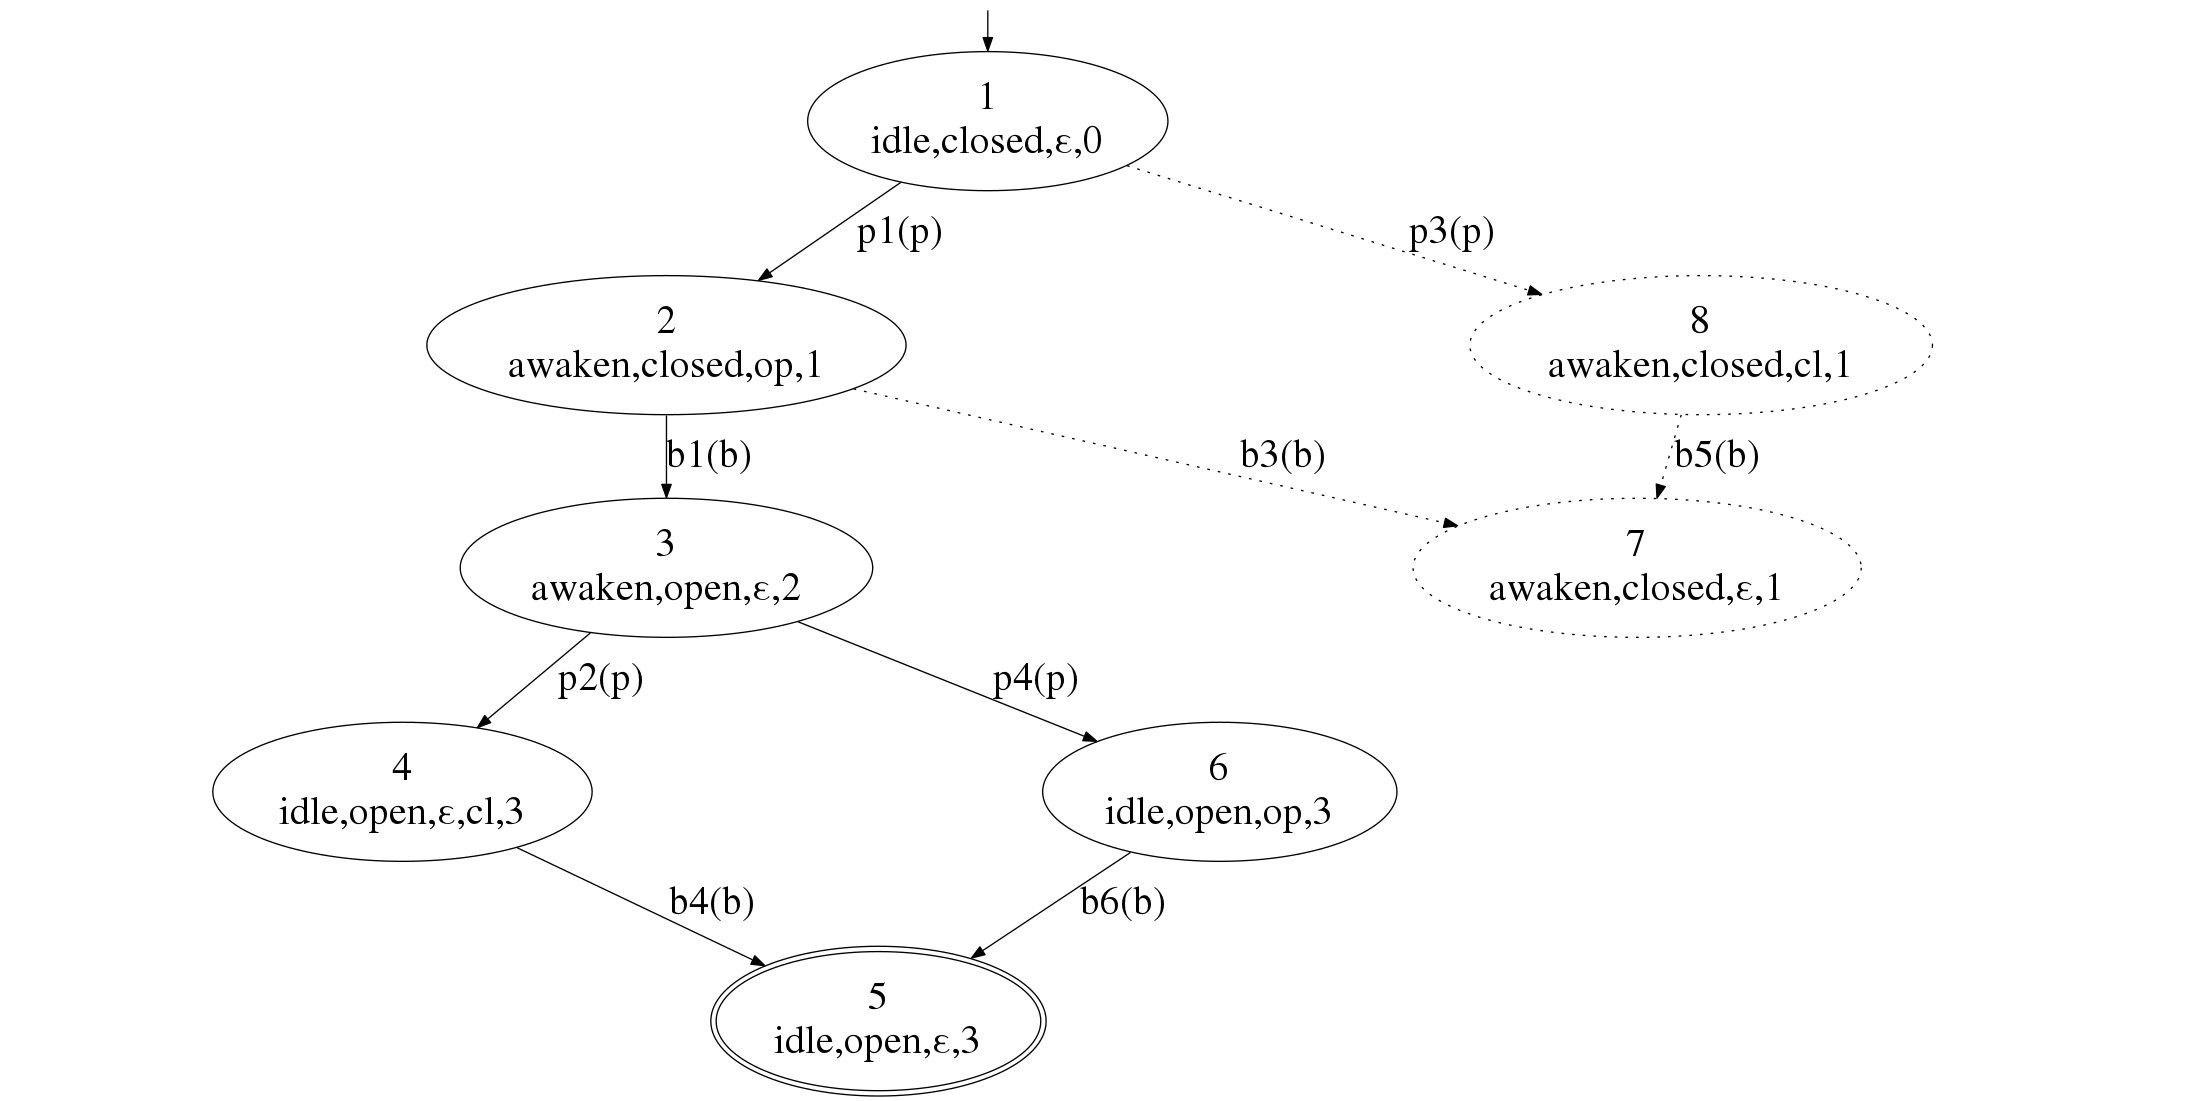
\includegraphics[scale=0.15]{./Img/sa/bhv_s.png}
\caption{Behavior del problema diagnostico $P(\overline{A})$. Le transizioni e gli stati tratteggiati indicano la parte spuria dell'automa}
\label{fig:bhv}
\end{figure}

\subsection{Decorazione del behavior}
Il secondo passo della ricostruzione monolitica consiste nella decorazione del behavior. Il linguaggio dell'automa ottenuto nel passo precedente è composto da stringhe, ognuna delle quali rappresenta una traiettoria consistente con l'osservazione temporale. Dato che il behavior racchiude tutte e sole le traiettorie la cui traccia rispetto al viewer è una traccia candidata dell'osservazione, la soluzione del problema diagnostico è l'insieme delle diagnosi relative a tali traiettorie. Dato che le traiettorie potrebbero avere dei cicli, dando luogo ad un numero infinito di percorrenze, l'idea è quella di marcare ogni stato del behavior con l'insieme diagnostico relative a tutte le traiettorie che terminano in quello stato. Il fatto di avere ciclicità non è un problema, poiché la percorrenza di più cicli non accresce la diagnosi già collezionata in precedenza. Il processo di marcare ogni stato con le relative diagnosi è detto decorazione.

\begin{defn}
Sia $Bhv(P(A))$ il behavior di un problema diagnostico $P(A)$. Il behavior decorato $Bhv^\star(P(A))$ è il DFA ottenuto dal behavior marcando ogni stato $\beta$ con un insieme diagnostico $\Delta(\beta)$ basato sull'applicazione delle seguenti regole:
\begin{enumerate}
\item lo stato iniziale è decorato con l'insieme diagnostico vuoto $\delta(\beta_0) = \{\emptyset\}$
\item per ogni transizione $\beta \xrightarrow{t(c)} \beta^\prime$, per ogni $\delta \in \Delta(\beta)$, se $(t(c),f) \in R$ allora $\delta \cup \{f\} \in \Delta(\beta^\prime)$, altrimenti $\delta \in \Delta(\beta^\prime)$.
\end{enumerate}
\end{defn}
La prima regola è quella base, in cui si associa alla traiettoria nulla la diagnosi vuota.
Se la decorazione di uno stato $\beta$ include una diagnosi $\delta$ allora esiste almeno una traiettoria $h$, che termina in $\beta$, la cui diagnosi è $\delta$. Conseguentemente, esiste una traiettoria $h \cup [t(c)]$ terminante in $\beta^\prime$ la cui diagnosi è $\delta$ se $(t(c),f) \notin R$, oppure è l'estensione di $\delta$ tramite la label di guasto $f$, associata alla transizione $t(c)$ nel ruler $R$. 
Quest'ultima regola è induttiva e deve essere applicata continuamente allo stato successivo della transizione fino a che la decorazione non aggiunge nuove diagnosi, raggiungendo una condizione di stabilità.
L'algoritmo di decorazione, in forma ricorsiva, è fornito di seguito (\ref{alg:decoration}).

\begin{algorithm}
\textbf{Decorate($Bhv(P(A))$)}
\begin{algorithmic}
\STATE Marcare lo stato iniziale $\beta_0$ con $\{\emptyset\}$ 
\STATE Marcare tutti gli altri stati non iniziali con l'insieme vuoto $\emptyset$
\STATE $Dec(\beta_0,\{\emptyset\})$
\STATE
\STATE \textbf{Function} $Dec(\beta$,$D)$
	\FORALL{transizione $\beta \xrightarrow{t(c)} \beta^\prime$}
		\STATE $D^+ \leftarrow \emptyset$
		\FORALL{$\delta \in D$}
			\IF{$(t(c),f) \in R$}
				\STATE $\delta^\prime \leftarrow \delta \cup \{f\}$
			\ELSE
				\STATE $\delta^\prime \leftarrow \delta$
			\ENDIF
			\IF{$\delta^\prime \notin \Delta(\beta^\prime)$}
				\STATE inserire $\delta^\prime$ in $\Delta(\beta^\prime)$ e in $D^+$
			\ENDIF
		\ENDFOR
		\IF{$D^+ \neq \emptyset$}
			\STATE $Dec(\beta^\prime, D^+)$
		\ENDIF
	\ENDFOR
\end{algorithmic}
\caption{Algoritmo di decorazione del behavior}
\label{alg:decoration}
\end{algorithm}

\begin{ex}
Con riferimento al problema diagnostico dell'esempio \ref{ex:problem}, in figura \ref{fig:bhv_star} è rappresentato il relativo behavior decorato.
Nella tabella \ref{tab:decoration} sono riportate le chiamate effettuate dall'algoritmo alla procedura ricorsiva $Dec$. L'ordine di considerazione delle transizioni è, rispetto all'automa del behavior decorato, da sinistra a destra.
\end{ex}

\begin{figure}[htbp]
\centering
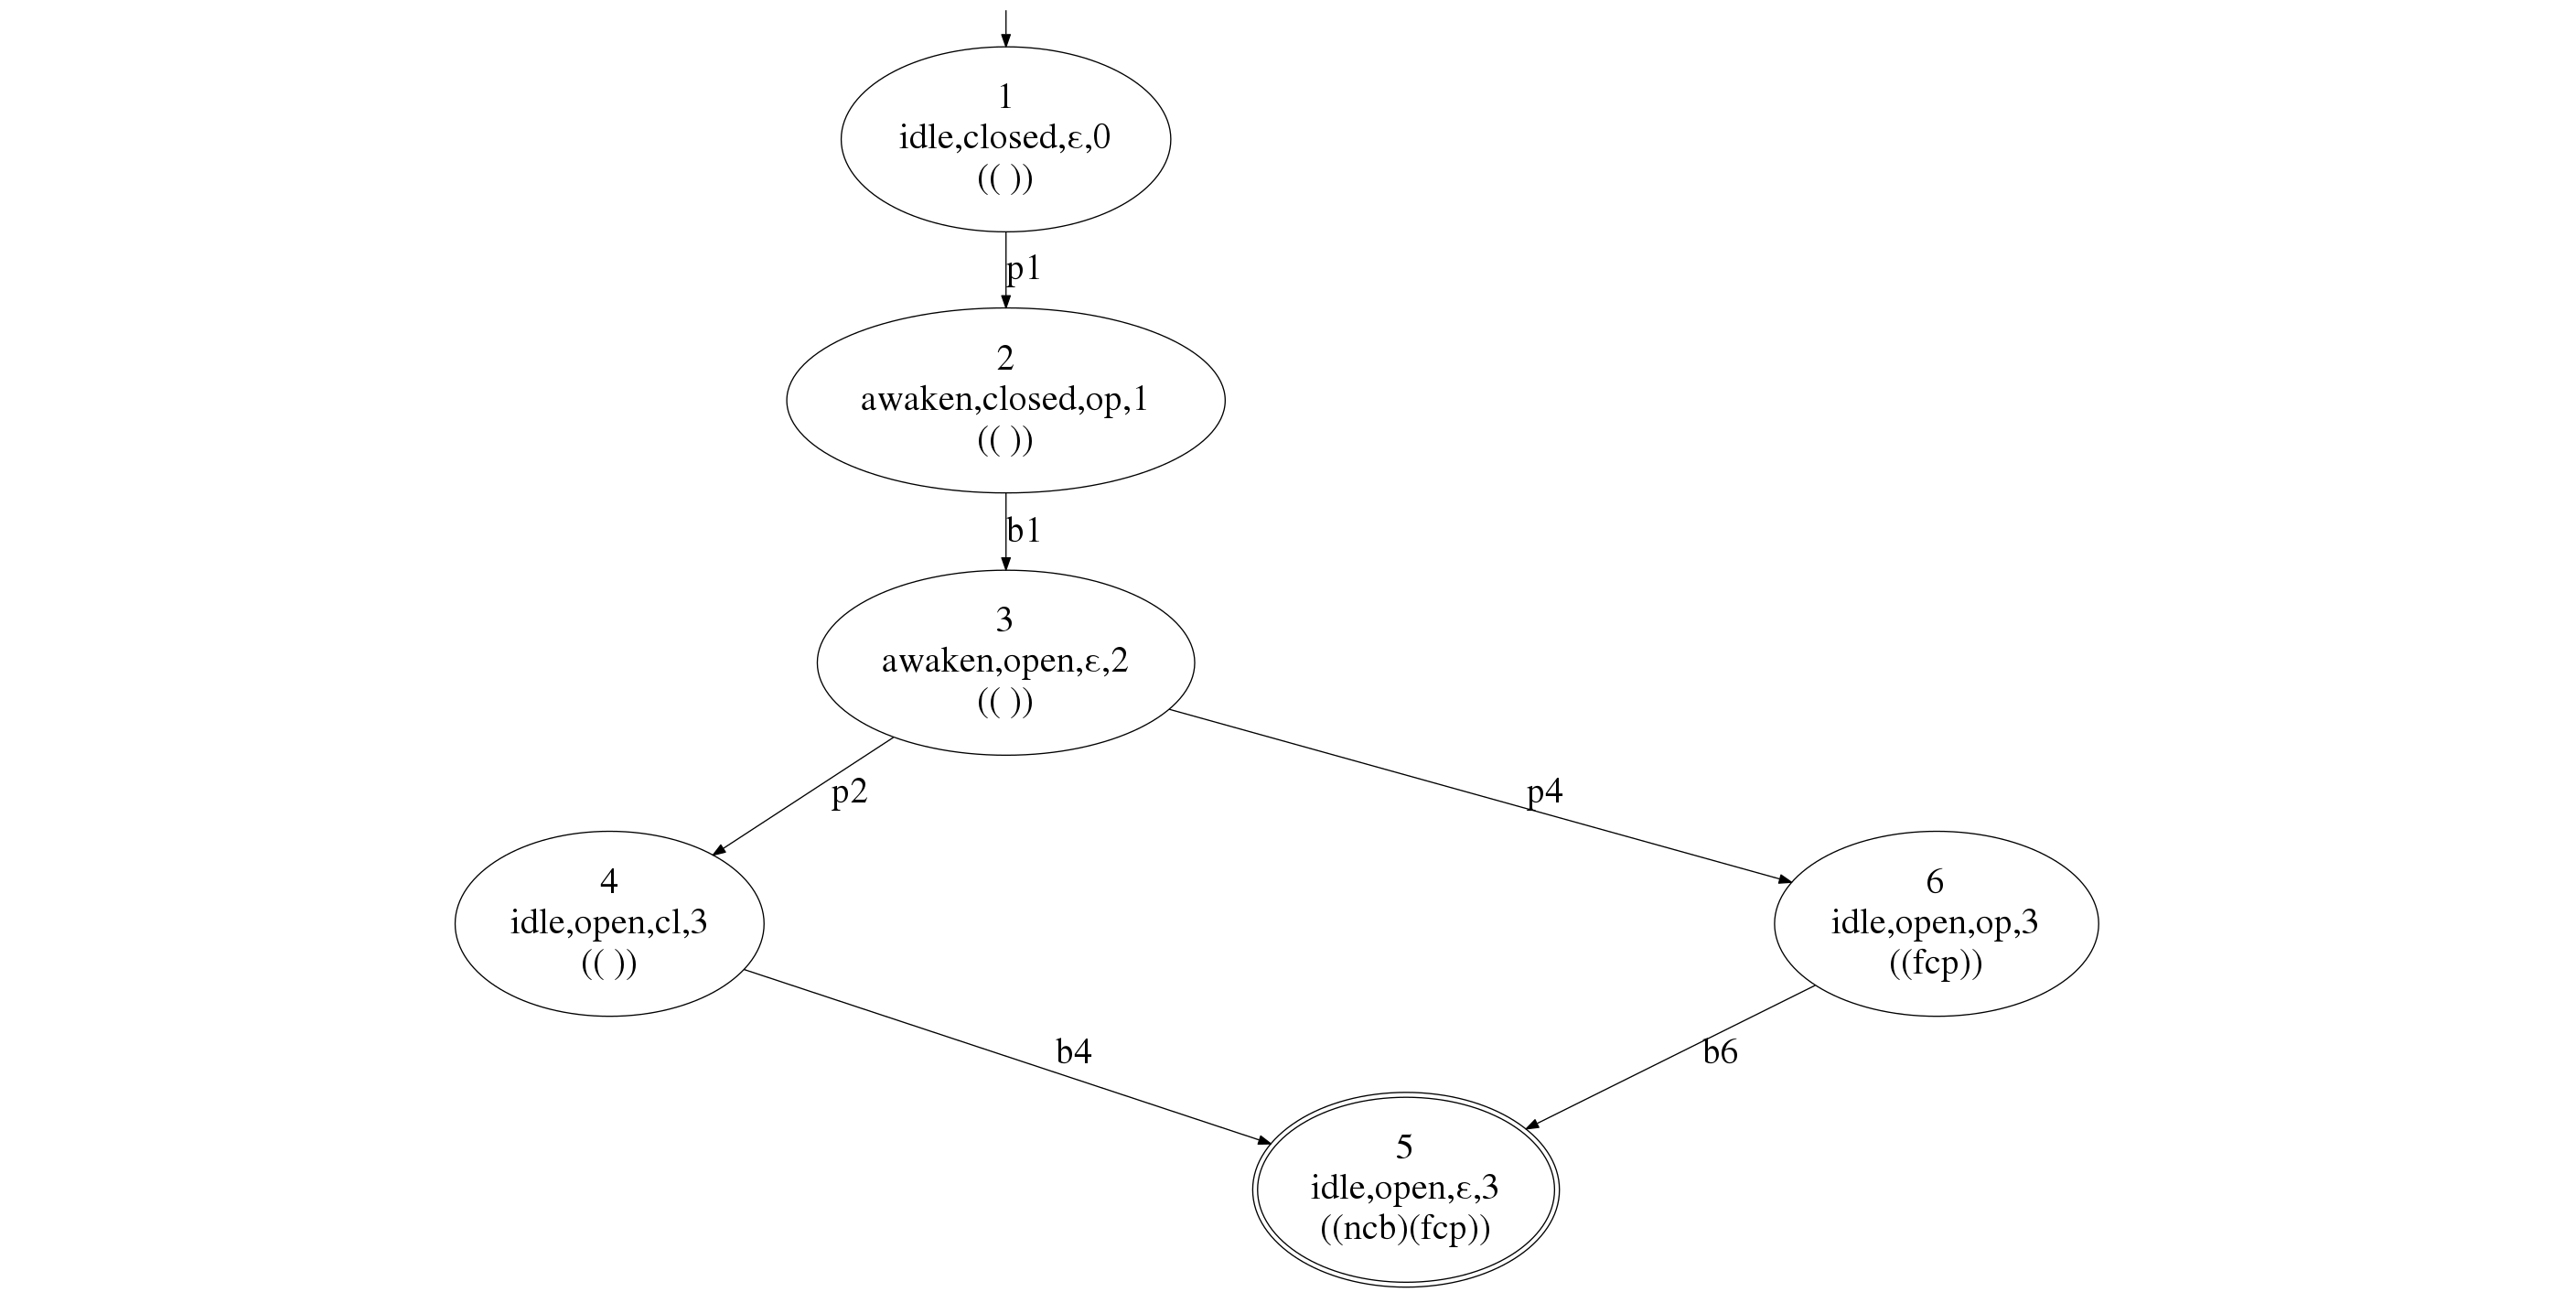
\includegraphics[scale=0.13]{./Img/sa/bhv_star.png}
\caption{Behavior decorato del problema diagnostico $P(\overline{A})$}
\label{fig:bhv_star}
\end{figure}

\begin{table}[htbp] 
\begin{tabularx}{\textwidth}{l c c c c c c c}
\hline
N & Chiamata & $\Delta(1)$ & $\Delta(2)$ & $\Delta(3)$ & $\Delta(4)$ & $\Delta(5)$ & $\Delta(6)$\\
1 & $(1,\{\emptyset\})$ & $\{\emptyset\}$  & $\emptyset$ & $\emptyset$ & $\emptyset$ & $\emptyset$ & $\emptyset$\\
2 & $(2,\{\emptyset\})$ & $\{\emptyset\}$  & $\{\emptyset\}$ & $\emptyset$ & $\emptyset$ & $\emptyset$ & $\emptyset$\\
3 & $(3,\{\emptyset\})$ & $\{\emptyset\}$  & $\{\emptyset\}$ & $\{\emptyset\}$ & $\emptyset$ & $\emptyset$ & $\emptyset$\\
4 & $(4,\{\emptyset\})$ & $\{\emptyset\}$  & $\{\emptyset\}$ & $\{\emptyset\}$ & $\{\emptyset\}$ & $\emptyset$ & $\emptyset$\\
5 & $(5,\{\{ncb\}\})$ & $\{\emptyset\}$  & $\{\emptyset\}$ & $\{\emptyset\}$ & $\{\emptyset\}$ & $\{\{ncb\}\}$ & $\emptyset$\\
6 & $(6,\{\{fcp\}\})$ & $\{\emptyset\}$  & $\{\emptyset\}$ & $\{\emptyset\}$ & $\{\emptyset\}$ & $\{\{ncb\}\}$ & $\{\{fcp\}\}$\\
7 & $(5,\{\{fcp\}\})$ & $\{\emptyset\}$  & $\{\emptyset\}$ & $\{\emptyset\}$ & $\{\emptyset\}$ & $\{\{ncb\},\{fcp\}\}$ & $\{\{fcp\}\}$\\
\hline
\end{tabularx}
\caption{Applicazione dell'algoritmo di decorazione per ricavare $Bhv^\star(P(\overline{A}))$}
\label{tab:decoration}
\end{table}

\subsection{Distillazione delle diagnosi}
Una volta che il behavior è stato costruito e decorato, la soluzione del problema diagnostico $P(A)$ può essere determinata calcolando l'unione delle diagnosi associate a stati finali del behavior decorato:
\begin{center}
$\Delta(P(A))) = \{\delta | \delta \in \Delta(\beta_f), \beta_f$ finale in $Bhv^\star(P(A))\}$.
\end{center}


\begin{ex}
Considerando il behavior decorato in figura \ref{fig:bhv_star}, la distillazione delle diagnosi avviene considerando l'insieme delle diagnosi relative all'unico stato finale $5$, cioè
\begin{center}
$\Delta(P(\overline{A})) = \{\{ncb\},\{fcp\}\}$
\end{center}
Si noti come la soluzione trovata è la stessa intuitivamente ricavata dalle definizioni nell'esempio \ref{ex:problem}.
\end{ex}